\documentclass[11pt]{article}
\usepackage[top=1.00in, bottom=1.0in, left=1in, right=1in]{geometry}
\renewcommand{\baselinestretch}{1.1}
\usepackage{graphicx}
\usepackage{natbib}
\usepackage{amsmath}
\usepackage{hyperref}
\usepackage{gensymb}
\usepackage{parskip}

\def\labelitemi{--}

\usepackage{fancyhdr}
\pagestyle{fancy}
\fancyhead[LO]{}
\fancyhead[RO]{}

\begin{document}
\bibliographystyle{/Users/Lizzie/Documents/EndnoteRelated/Bibtex/styles/besjournals}
\renewcommand{\refname}{\CHead{}}

%%%%%%%
%% To do %%
%%%%%%%

% Test data code for y = ax + b?
% Ask WDP to add prior rants
% https://github.com/lizzieinvancouver/gelmanhill/wiki/Vocabulary

\title{How to fit Bayesian models and influence people \emph{or}\\
How to do Bayesian model fitting in ecology \emph{or}\\
The best way to be a Bayesian in ecology today}
\date{\today}
\author{EM Wolkovich and WD Pearse and TJ Davies and M Betancourt?}
\maketitle

% 160 words; main text is 4,000
\abstract{Improvements in algorithms and computational speed have heralded a new a era of Bayesian model fitting. Models are easier to fit, faster to run, and more flexible, making them ideal for many of the complexities of ecological sampling designs. This has opened up Bayesian approaches to a new world of users, but how best to start using and implementing them in ecology is still somewhere between old rules and methods and the new schools of Bayesian analysis. Here we present a Bayesian workflow---centering on model and data simulation---that represents a ground shift of not just how to do fit Bayesian models, but how we should approach statistical model fitting to advance our science. This workflow integrates mechanistic and statistical models with a computational toolkit, which we argue could accelerate ecological science. Steps of this workflow will often highlight current limits of our inference---as they provide a clear method to test how uncertain models are given small sample sizes, or how often a poor model may appear `best' given certain diagnostics---and thus also provide the path forward. By interrogating our methods through generative models and data from such modes, we can refine where to put resources for better estimates, better models, and better forecasts. While we outline these methods from the happy surf of our Bayesian beach, the ocean we describe works for anyone fitting models to ecological data. 
% Maybe along the way we highlight common practices in ecology that are stupid as all tomorrow---as our approach makes clear---and outline best practices for jumping into the wonderful surf of the happy Bayesian ocean. %JD16Aug: Obvious bad practices: small sample sizes and forking paths, thresh-holding on p-values, model selection and minimum adequate models etc.

\section{Main text}
\setlength{\parindent}{0pt}
\setlength{\parskip}{7pt}


Recent years have seen the explosion of Bayesian models across fields \citep{vandeschoot2021,schad2021,grinsztajn2021}, including ecology. This change comes in part from increased computational power, but more from new algorithms \citep[e.g. Hamiltonian Monte Carlo,][]{nuts2014,betan2019} that have made Bayesian models faster and arguably easier to fit \citep{Carpenter:2017stan}. Capitalizing on these advances \textsf{R} packages, such as \textsf{brms}, have seen much wider use than the previous generation of packages that streamlined fitting a set of pre-determined models using Bayesian approaches (e.g. \textsf{MCMCglmm}). Bayesian approaches, long heralded as more powerful, flexible and especially adept at capturing the multiple levels of variance in ecological data, seem poised to help ecology as a discipline advance in leaps and bounds, and to avoid contributing to the replication crisis.

Ecology itself also seems poised to leap out of the jungle and into the role society is asking of it as growing global challenges demand more predictive models of how communities and ecosystems will shift with climate change, habitat degradation and other anthropogenic forces. Ecology, now three decades on after the start of the synthesis movement, has greatly advanced its statistical and computational approaches to test fundamental theory across systems \citep{Hampton2013}. Early concerns have given way to a widespread appreciation of the value of these new approaches (alongside a resounding and bizarre fervor over `natural history'). At the same time, growing anthropogenic challenges have increased the need for predictive models and forecasts from ecologists. [JD adds: models that embrace uncertainty, something we still find hard to communicate well, and variability vs mean responses...]

The result is that the average ecologist today has a diversified skillset compared to that of decades ago. Ecology has long been a field with deep statistical training, but in many ways the modern ecologist is now also expected to be computational---able to handle large datasets, produce repeatable workflows, and help translate models into forecasts for policy and planning. Many ecologists now bridge field, lab and computational methods. Bayesian methods can help facilitate this new job description. % As such, the rise of Bayesian approaches is especially timely for ecology. % The average modern ecologist is computational, but often grounded in the natural history of a particular system (err, maybe, on both these accounts, but whatever).

Bayesian approaches are in not to ecology, as they have long been used in certain subdisciplines related to estimating population sizes of things people want to eat or manage. For example, wildlife biology widely uses mark-recapture data and associated models to estimate population sizes; these methods almost always use Hidden Markov models, which can rarely be fit without Bayesian methods \citep{muthuku2008,zheng2007}. Similarly, fisheries biology has tended towards more complex models---such as state-space models---to estimate stocks, which are similarly easiest to fit with Bayesian approaches \citep{trijoulet2018,millar2000}. % For decades, Bayesian training in ecology has focused on these aims, but as data and methods change, so has how ecologists are using Bayesian models. 

However, away from these fields, ecologists have largely focussed on frequentist statistics, null hypothesis testing, and p-values. [perhaps mention part of the appeal of these methods come from their ease of interpretation, a t-test provides a simple summary statistic to the question of whether two groups are different.] However, underlying assumptions on the assumed distribution of data are often ignored, spatial and phylogenetic data introduce non-independencies, and in large ecological datasets we often fit multi-way interaction terms that make main effects hard to interpret, or random effects to correct for group level factors. The arguments for simplicity start to become weak.

Today, as large-scale ecological data becomes available for more diverse systems and for questions addressing other aims, ecologists are using Bayesian models in new ways. Yet, there is naturally a lag in training in statistics, and in Bayesian modeling in particular. Bayesian approaches provide a pathway to powerful models that can transform how we understand our systems, but they can also lead to pitfalls most ecologists are not trained to notice or deal with. Many of these pitfalls can be avoided by approaching Bayesian analyses through specific workflows \citep{betanworkflow,vandeschoot2021}, which themselves are built on a process of how to do not just stats, but how to do science. 

Here we describe a broadly generalizable workflow for Bayesian analysis and show how it can revolutionize training in ecology by integrating more model building and model understanding. Once you start doing this workflow, your scientific life will never be the same. 
%  allow fitting complex models without much influence of the data fed into the model. 

\subsection{Box by WPD with 3-paragraph explanation of Bayes}

Someone with the initials WPD will hopefully write this. 

\subsection{A brief overview of the benefits---and pitfalls---of Bayesian models} 

Bayesian models have many benefits, but an often-mentioned one is that `you can fit any model you want.' While this is not entirely true \citep{BDA,reid2019}, compared to the models ecologists can fit in popular modeling packages (e.g. \textsf{lme4}) Bayesian modeling options can feel limitless. As long as you can write out the likelihood of your desired model and assign priors to all parameters, you can generally `fit' any model. This includes non-linear ones, non-Gaussian families (e.g. Poisson, beta or combinations thereof, such as hurdle models), hierarchical designs and any combination of these, as well as `joint' models where parameters estimated in one equation appear in another, thus carrying through estimated uncertainty. Such flexibility is incredibly powerful in ecology where data are often influenced by complex spatial or temporal patterns, non-linear processes are widespread and common data types, are non-Gaussian (e.g. counts, percent cover etc.). 

%JD16Aug -- `we often really want ...' I think this is an important point that could be expanded - what is the point of fitting models - we want to know the effect of something on something else (this is especially important in e.g. pharmacology and global change biology).
Fitting a bespoke model to your data allows us to get the numbers we often really want but don't have access to. Thus, instead of reporting a treatment's $p$-value and accompanying F statistic and degrees of freedom, models can be designed to estimate and report effects per \degree C of warming or at what level non-linearities due to high temperature begin---always with estimated uncertainty. While replication crises in other fields, driven in part by a overly zealous focus on $p$-values \citep{halsey2015,loken2017}, and the rise of meta-analyses in ecology \citep{Hampton2013} have led to a somewhat greater focus on `effect sizes' in ecology (often used to refer to very specific unitless statistics, such as Cohen's $d$), bespoke models take this to a new level. Researchers can easily estimate comparable effect sizes from z-scored data (in units of standard deviation), alongside estimates in meaningful natural units, such as per \degree C of warming or per hectare of habitat lost. 

% JD16Aug -- is this really one the biggest pitfalls of B? It does not seem so bad, in fact Bayesian seems well suited to such models ... perhaps a bigger issue is mispsecified models, especially when data are complex and you fit a bespoke model.
But this valuable flexibility is also one of the greatest pitfalls of Bayesian models. You can fit almost whatever you want, but critical parts of your model might be almost entirely unimpacted by your data. And in ecological model fitting, we're currently most often interested in parameter estimates strongly informed by our data. 

% JD16Aug -- I think we need more pitfalls of Bayesian ...
This `pitfall' of Bayesian is not new, nor unique to ecology---though the complexity of ecological data and processes may make it especially pernicious in ecology---and decades of statistical research has aimed to develop best practices when using Bayesian models to avoid this. These best practices generally center around a specific workflow; a variety of which can be found in exquisite detail elsewhere \citep{betanworkflow,grinsztajn2021,vandeschoot2021}. We do not aim to repeat those here, but instead to provide a highly simplified---but powerful---workflow that, when applied to Bayesian modeling in ecology, could greatly accelerate progress. % This is a short overview of a much deeper topic. See \href{https://www.nature.com/articles/s43586-020-00001-2}{Bayesian statistics and modelling} for a little more depth, including how to develop priors and your basic model formulation.\\

\subsection{A very basic Bayesian workflow}

We outline a Bayesian workflow below that includes what we consider the major steps for Bayesian model fitting (Fig. \ref{fig:workflow}). Many steps should be familiar to statistical ecologists, but are often overlooked, whereas other steps may appear particular to Bayesian (e.g. prior predictive checks), but are actually useful for anyone---using Bayesian models or not---to challenge their models of how the world works. 

As we focus on a simplified list of major steps, many of the smaller but still critical steps are omitted. For example, visualization is required at every step---especially 2 and 4; while we do not discuss this explicitly we refer to relevant publications. We also jump in, and somewhat over, one of the biggest steps. 

We present the workflow assuming users have a model already in hand, which---if you have collected data---is true. Your model may be only verbal or conceptual; however, for this workflow, you'll need to convert such models into mathematical versions. This can be challenging at first, as ecologists often learn only a simplified version of this step (often focused on identifying which distribution---normal, binomial, zero-inflated Poisson, etc.---their response variable most closely resembles), and approach it after data collection. In reality, skilled users of this workflow will develop their model before they collect and refine it---or develop possible additions to it---as they collect data; models often fit best when they include both the underlying biological model being studied and a model of the data generating process (e.g., gaps between sampling dates, biases in sampling etc.). 

Getting to the point where the Bayesian workflow is part of data design and collection, however, requires starting somewhere---with some model in hand. A suite of resources on generative modeling can help \citep{statrethink,betangen}, along with two points. First, you must start somewhere, so know that you can and will improve on this skill. Second, as you start, ask lots of questions---and push yourself on your answers---what do you expect and what's reasonable biologically from your model? For example, instead of simply identifying to which distribution your response variable looks most similar, ask yourself what generates that distribution and what you think its mean, minimum and maximum is. Do you expect data below zero? Up to infinity? If not, why not? You'll be generating your model---including its priors---as you do this. 

Our workflow is explained mostly program-agnostically. Though at times we assume a user of \textsf{Stan}, a relatively new probabalistic programming language, that interfaces with \textsf{R, Python, Julia} (and more) to write bespoke Bayesian models and underpins the \textsf{R} packages \textsf{brms} and \textsf{rstanarm}, which fit a suite of specific (pre-defined) models \citep{Carpenter:2017stan}. We focus on \textsf{Stan} as its MCMC algorithm (a variant of Hamiltonian Monte Carlo, HMC) is fast and produces specific output to warn of model fit issues (i.e., divergent transitions) in a way other MCMC algorithms do not (e.g. Metropolis-Hastings or GIBBS), but the basic workflow should apply to diverse implementations of Bayesian modeling. \\

\emph{Step 1: Check your model code.} \\ 
% This obvious step assumes a suite of crucial work already done to define your model of interest. You must understand your question, your subdiscipline, and your data enough to formulate a useful model that you want to fit. This step thus assumes you arrive with a wealth of scientific expertise and a well thought-out model. 
To start the workflow, you need to write up your model and check it. As with all code, just because it runs, does not mean it does what you think it does. Whether writing it out in \textsf{Stan}, where you need to be able to write out the full likelihood and set all your own priors, or using a package that writes much of the model for you (e.g. \textsf{rstanarm}), you need the code and a way to verify the code is correct---test data.

Test data (aka `simulated data', or  `fake data,' etc.), and the skills required to build it, are central to this workflow. The idea of `test data' is that you simulate data from your model in such a way that you can use the resulting data to test your model code is correct. This means that to build test data you need to understand your model well enough to generate data from known parameters (which you select); you then run that data through your model and confirm it returns the parameters. %  As the goal is to test your model code, you'll want test data that is well-replicated, balanced and otherwise ... (err, actually -- skip this -- as it assumes a model without a data generating process in some ways). 

This very basic model checking step is uncommon for many ecologists, but critical in our view. If you can simulate data from your model, then you can powerfully---and easily---answer questions related to statistical power, what effect sizes are reasonable, and---most likely---have new insights into how your model suggests the world works. `All models are wrong; some models are useful,' becomes much clearer when you have the power to generate data from your model under any parameter set you want. Conversely, if cannot complete this step, you'll struggle to understand if the model fit well, and struggle further to meaningfully interpret the model output, making this apparently simple programmatic step actually encapsulate a far deeper understanding of your model. Once your \textsf{Stan} output returns the parameters you expect from your test data, you can move onto interrogating your priors. 

%JD16Aug -- Step 2. Set your priors (you know more than you think).
%JD16Aug -- Step 3. Check your priors
\emph{Step 2: Check your priors.} \\
Priors are the source of much discussion and focus by Bayesian and non-Bayesian researchers alike. Often treated as the big bad wolf of Bayesian, or the unseen hand producing the model fits you get, according to some. More accurately they are half of the equation that gives you your model posterior; and they are \emph{designed to be that way}. Bayesian philosophically is built around the idea that you have prior knowledge that you trust and want to compare to new data (with your new data showing up through your likelihood).

How much priors influence your model fit is in many ways up to, and your data. Depending on your model and the data, the likelihood (influenced by your data) can easily overwhelm your priors.  On the other hand, as you can fit a Bayesian model with 100 parameters and only 5 datapoints, there can be cases where your priors matter a lot. Most dangerously, failing to think about them, check them and understand your model enough, can mean they may matter more than you know. %JD16Aug --  Dolph always compares the 'danger' of priors in the belief that Saddam Hussein had WMDs - data was sparse, so priors overwhelmed. Han Solo flying the Millennium Falcon through an asteroid field illustrates the benefits of priors. We need to know where we are on the Saddam - Han spectrum.

Luckily you can use the code that you wrote to build test data (Step 1) and can use it for prior predictive checks. In these, you explore a distribution of potentially reasonable values for your priors, then see how they influence your resulting output. How exactly to do this depends on your question, model and aims, but many guides can help you think through this \citep{betanprior,wesner2021,winter2023}. 

In our experience, prior predictive checks can quickly disabuse newbies to Bayesian skeptics of their prejudices.  For example, you may not think you have a prior on how sunlight affects plant growth, until you realize your `agnostic prior' actually allows plant growth of hundred of meters per day for one individual plant. Prior predictive checks in this way serve both as a check on the priors you're using, and to further explore the model of the world to which you're planning to fit your data. % JD16Aug -- This is more about setting your prior (my step 2) than checking your prior - perhaps it does not matter if your prior allows plants to grow 100m per day. 
 
 \emph{Step 3: Run your model on your empirical data.} \\
The next step is to run the model---you've now validated, test-run and have ready to go---on your exciting new empirical data. Check diagnostics so you know it's running well and adjust until it is; this includes a suite of convergence and efficiency metrics ($\hat{R}$, ESS, lack of divergent transitions etc.) that are well-discussed elsewhere \citep[][and not our focus here]{betanworkflow,gelman2020bayesian,vandeschoot2021,gabryvis}
 
This is the step many ecologists skip straight to, ourselves included. It's easy to see the appeal---fitting our new data to the model can feel like the moment when we'll learn something new. But, at least in our experience, this is not always the case. When we rush to this step, that first model we fit is often followed by another, and another---perhaps because one does not converge, or the results of another do not make immediate sense. After a while of this process, it can easily feel like we're not sure what we learned, if anything. And we can get distracted from what we are actually most interested in---the biological effects. In contrast, by approaching the model through Steps 1-2, it's often much easier to quickly see through the results of the model fit. And also easier to plan next steps. 
 
% This is the step many ecologists skip straight to, leaping over steps 1-2 without realizing all they are missing along the way. While we can understand this approach---given the excitement of wanting to see how new data influences the model---we hope it's now obvious how much more can be gleaned from data by approaching the model through Steps 1-2. 
%  As we're all familiar with this step, it's hopefully straightforward. Run the model---you've now validated, test-run and have ready to go---on your exciting new empirical data. Check diagnostics so you know it's running well (convergence metrics, lack of divergent transitions etc.) and tweak until it is. 

 \emph{Step 4: Retrodictive predictive checks} \\
Once you have your posterior based on your model and new empirical data, it's time to interrogate it. Steps 1-2 have set you up well for this, as you have a sense of what different parameter estimates do to the model. 

% JD16Aug -- I feel there needs to be clearer justification on why we should do this. I have my model estimates, what more do I need?
Now that you have the parameter estimates from your posterior you can simulate new data from them and see how that new world looks to you---called retrodictive predictive checks (or posterior predictive checks, Fig. \ref{fig:retrodictivecheck}-\ref{fig:retrodictivecheckSD}). Exactly how to do these are---again---dependent on your question, model and aims \citep[but there is lots written on this,][]{held2010,gelman200ppc,conn2018}. In contrast to prior predictive checks, however, this step is built into some software. If you use \textsf{rstanarm}, then the package \textsf{shinystan} will automatically give you a set of retrodictive predictive checks, including comparisons of the mean and variance of simulated datasets with those of from your empirical data. Often here you may find big differences from your empirical data, and can start to generate hypotheses for why.

% \emph{Feedbacks in the workflow}\\
With those hypotheses in hand, you may very well want to tweak your model---this is all part of the workflow. At that point you return to Step 1, tweak your code, and repeat the process. In this way, fitting multiple models is encouraged, but in a far more structured and careful way than traditional ecological model fitting in our experience. And there are big benefits to it. % JD16Aug -- make clear this is not the same as model comparison or searching for a best fit model (although there are ways to compare models without overfitting, e.g. LOO)

This process more fully integrates mathematical modeling into statistical modeling. To complete Step 1, you have to understand the underlying math of your model enough to simulate data from it. This can be challenging at first (e.g. in our courses many students cannot recall how to simulate $y$ data for a simple linear regression), but is immensely beneficial to understanding your model. Indeed, we have found the greatest insights come not from the step we all know best---fitting the model with empirical data---but from every other step in this workflow. Developing simulated data to test the model, running prior and retrodictive checks all dive you deep into understanding your statistical model, which suddenly you may find yourself thinking through much more mechanistically. In our experience this process has quickly translated into insights for our biological systems, and changed how we approach statistical models. 

\subsection{How this workflow changed our science} % Surprising things that happened to us that may happen to you if you follow this workflow
% JD16Aug -- I wasn't sure I was going to like this section, but you won me over - I just struggled with the 'simplify' section a little 

As we have used this workflow, how we approach our statistical models has changed. These changes have generally been similar for each of us. We suspect they are not unique to us, our study systems or questions. Instead, we think they represent common approaches to statistical modeling in ecology that could help the field progress, much as we believe they have helped our science advance. 

 \emph{Understanding nonidentifiability} \\
Identifiability and---more common in our experience: nonidentifiability---refers to when all parameters in a model can be uniquely identified. Models can be nonidentifiable in several ways, including when mathematically some parameters cannot be uniquely defined. Statistically, nonidentifiability often is an outcome of the empirical data combined with the model. In this definition nonidentifiability occurs when the data do not contain ``sufficient information for unique estimation of a given parameter or set of parameters in a particular model'' \citep{gelmanhill}. 

Nonidentifiability can come up in many ways in ecology---and be hard to see, especially if you rush through model fitting. But if you have to write out your model and simulated data, you may suddenly realize lots of places for nonidentifiability to live. For example, when species do not occur across most sites, a model including separate parameters for site and species is often nonidentifiable, but there's no warning in packages to tell you this; you have to learn it from the data. We have become far better experts at nonidentifiability based on this workflow---and we have adjusted how we collect data and interpret results because of it. % JD16Aug -- and sometimes it doesn't matter if your are interested in the effect of a separate parameter.

 \emph{Simplify} \\
Once we noticed how pervasive nonidentifiability and weak identifiability (where parameter estimates are highly uncertain because the model and data together are nearly nonidentifiable) were we started simplifying our models. Whereas previously when we had data that qualitatively appeared complexly nested, crossed, split or twisted, we would have tried to fit all of these intricacies (on the intercept) we are now more slow to add these to our models. By both understanding these terms better (including the many different ways each can be modeled), and understanding them better---depending on the data and model in each unique context---we work more carefully through what to include. % JD16Aug -- I feel there is a tension between the philosophy of 'if you think it might be important, then include it in your model' and make your model simple. We want both. But perhaps all those crazy interaction terms that are impossible to make sense of could be ignored ... 

% JD16Aug -- this was even referred to as 'model simplification' and we searched for MAMs (minimum adequate models) - See Crawley.
Before using this workflow, some of us would start with complex models, then simplify models until they converged. Often these were hierarchical models with many levels, built based more on a dogma of non-independence (and, somewhat relatedly, correct degrees of freedom) than an understanding of the model. We also often fit a suite of interactions: multiple two-way interactions and the occasional three-way interaction were common fare. But in simulating data, and fitting models to real, messy, imbalanced data using the workflow we came to see how much we were asking of our data and models together. Fitting a two-way interaction with half the effect size of a main effect takes a 16X sample size, compared to fitting the main effects alone \citep[which then average over the interactions][]{regotherstories}. This is sobering. It's more sobering when you see it played out again and again through this workflow. % JD16Aug - I have always been a bit confused about this. If the interaction term is important, surely it is still better to try and include it in the model even if we can't estimate it? Perhaps this is a difference between analysing observational vs experimental data (where we can set the sample size).

We now simplify based on a more careful reckoning. Usually this starting model is not simple, it often includes grouping factors that may be difficult to fit, but that we see as absolutely critical to the question, model and data at hand. We build up from there, often grouping posteriors by some factor (e.g. site or biome) before we add it to our model. 
% JD16Aug -- (prev sentence) -- This part I would stick under your step 4 - predictive checks don't look good, likely because we are missing something ...
However, the ending model is often not as complex as we may have fit if we did not follow all the steps. 
% JD16Aug -- (prev sentence) Really? I tend to just leave it in and say it doesn't matter ...
And---through them, especially Step 4---we can feel confident our model is capturing important variation. 
% Once you do the workflow, you may end up like us: fitting fewer levels in your mixed effects models, fitting fewer interactions.

Understanding this variation includes re-approaching how we plot our model and data. While many of us are good at plotting raw data, and plotting our main model parameters (and plotting both these pieces together), the world in between is rarely taught. And it's in this in-between world that we have found a deep understanding of our models, what they're doing and---relatedly---what our results show. Many packages offer model predictions---based on a full or near-full model, but being able to decompose model predictions into varying components can give powerful insights. For example, model predictions can be plotted with and without major grouping factors such as `block,' `plot', or `species,' and suddenly how predictable a model is (or not) based on other factors like `treatment' or `time' becomes clear. 

 \emph{Looking at parameters, not p-values} \\
Before this workflow, not all of us commonly discussed the values that parameters in our model took---things like the slope and intercept (two common model parameters) were sometimes reported, but we did not know them as well as we knew whether the $p$-value for the slope was $<0.05$. This changes quickly when you need to build simulated data, for example, for a phenological event (a day within the calendar year so, ideally between 1 and 366) and suddenly find it's $>$1000 based on the quick parameters you put into your code. 

This focus on the value of parameters scales up through the workflow and across projects. Having a better sense of parameter values across different biological contexts, model parameterizations, and time periods gives a better sense of how the biological world works, including what's reasonable, possible or wildly unrealistic. % Suddenly, weakly informative priors make ever more sense .... 

\subsection{How this workflow intersects with ecological training} %Challenges of the workflow compared to how we traditionally train ecologists

This four-step workflow is a simplified version of the current best practices for Bayesian model fitting  \citep{betanworkflow,vandeschoot2021}, but many of the skills required are not part of traditional ecological training. Writing out the math behind most statistical models enough to complete Step 1 bleeds into the skillset usually reserved for those working on theory, where coding and simulating from a model are common tasks. In contrast field, lab and otherwise empirical-data based ecologists often fit models they could not simulate data from. This dichotomy seems short-sighted in our current era, of bigger, messier data and greater computational methods poised to handle such messy data---if scientists are trained in how to build the right models for their questions and data. A reasonably competent coder could easily simulate data under a complex model that they might not have the mathematical expertise to solve. % We believe training ecologists with a skillset where they quickly can use this workflow could advance ecological science rapidly. % Theory = simpler models = outcome of a good Bayesian workflow (often)

This workflow also requires a shift in how we approach Bayesian methods---and training in Bayesian models---in ecology. Already, uptake of new Bayesian \textsf{R} packages highlight that Bayesian methods are no longer the purview of only wildlife and fisheries biologists, and these changes come alongside advances in Bayesian workflows, algorithms, and visualiziations \citep[e.g.][]{betanworkflow,vandeschoot2021,gabryvis}, that ecology must adapt its training for. While this is an active area, we highlight three major changes.

(1) Prior `beliefs' are changing. Best practices for determining priors is an active area of statistical research \citep{BDA,regotherstories}, and training should reflect current best practices. These include that `non-informative priors' are a misnomer, as they are often informative  \citep{lemoine2019}, and priors can easily be `weakly informative.' Thus a strong focus on the dangers of priors in training can be overkill (see supp or box where WDP includes part of his rant?). 

Current training often includes a very strong focus on priors, including conjugate priors, because of the importance of conjugate priors in closed form solutions for particular posteriors. Modern algorithms, such as HMC, do not require conjugate priors, which are now antiquated (and thus sometimes referred to as  `the crystal deodorant of Bayesian statistics'). Prior predictive checks provide a far more powerful way to understand how priors work within a particular model, and are far more useful than rules about which priors should be fit in certain cases or memorizing which priors are conjugate. 

(2) `Random effects' are not just random. Hierarchical models contain grouping factors, sometimes referred to as `random effects,' such as species or individual. This term, however, is misleading, imprecise and thus no longer recommended \citep{gelmanhill}. In ecology, it also carries with a heavy weight of older `rules' of what is `random' versus `fixed,' including that `random effects are things you don't care about (for example the `block' effect from a randomized block design). After retrodictive posterior checks (Step 4), you might feel differently, as hierarchical effects are (by definition) drawn from an underlying distribution---meaning you can predict outside of the specific set you sampled (for example, you can predict for a new species or individual), whereas you cannot do so for most `fixed effects.'  % JD16Aug --Hmm I am not sure I buy this, unless you are suggesting comparing species as a grouping factor vs fixed effect (rather than  a random effect)

(3) P-values are easily misleading (\href{https://www.youtube.com/watch?v=c3hxhv0lpI0}{`I am arbitrary but my story is often told ... '}), and there's no easy fix for that. The replication crisis, rampant in other fields, is based in part on an overly hopeful belief that $p$-values will separate the signal from the noise, with one easy number. In reality, small sample sizes, lack of routine reporting of interpretable effect sizes, fitting of many models without adequate explanation, poor data and code reporting habits all increase the chance of finding `significance' at a level of $\le0.05$ \citep{halsey2015,loken2017}. This reality means a similar crisis is likely lurking in ecology, especially given small sample sizes alongside a tendency to fit complicated models with multiple interactions. The answer to this, however, is not to make p-values smaller \citep{halsey2015,colquhoun2017}, nor is it Bayesian approaches , which (as we touch on above), bring their own ways to sift exciting results from a pile of chafe. 

The answer is a workflow for careful model building, model fitting and model interrogation---as we outline here. %Try it, and see if it transforms your life they way it transformed ours!
This workflow depends strongly on simulating data---for testing your model (Step 1), testing your priors (Step 2) and understanding your model (Step 4)---an area we actively under-train in ecology. This workflow makes clear how relevant and important simulation is, but the relevance of simulation extends well beyond Bayesian model fitting. As larger datasets and machine learning increase their utility, and prevalence, methods to test our understanding, interrogate our models and develop new models, will depend strongly on simulation, potentially transforming ecology, as it is transforming science in general \citep{flynn2022digitaltwin,kuntz2022,oren2017}.

\iffalse
\subsection{Conclusions}
\begin{enumerate}
\item Ecologists cannot simulate their stats (or simple systems for that matter). Evolutionary biologists can. (And the field is better for it.)
\item Maybe hint at that you need these skills (and unit testing) given rise of AI?
\end{enumerate}
\fi 

{\bf Take home messages (maybe)}
\begin{enumerate}
\item You should not fit a model you cannot simulate
\item Fit simpler models
\item Know your nonidentifiability
\end{enumerate}

\newpage
\section{References}
\vspace{-5ex}
\bibliography{refs/bayesrefsmini.bib}


\newpage
\section{Figures}

\begin{figure}[ht]
\centering
\noindent 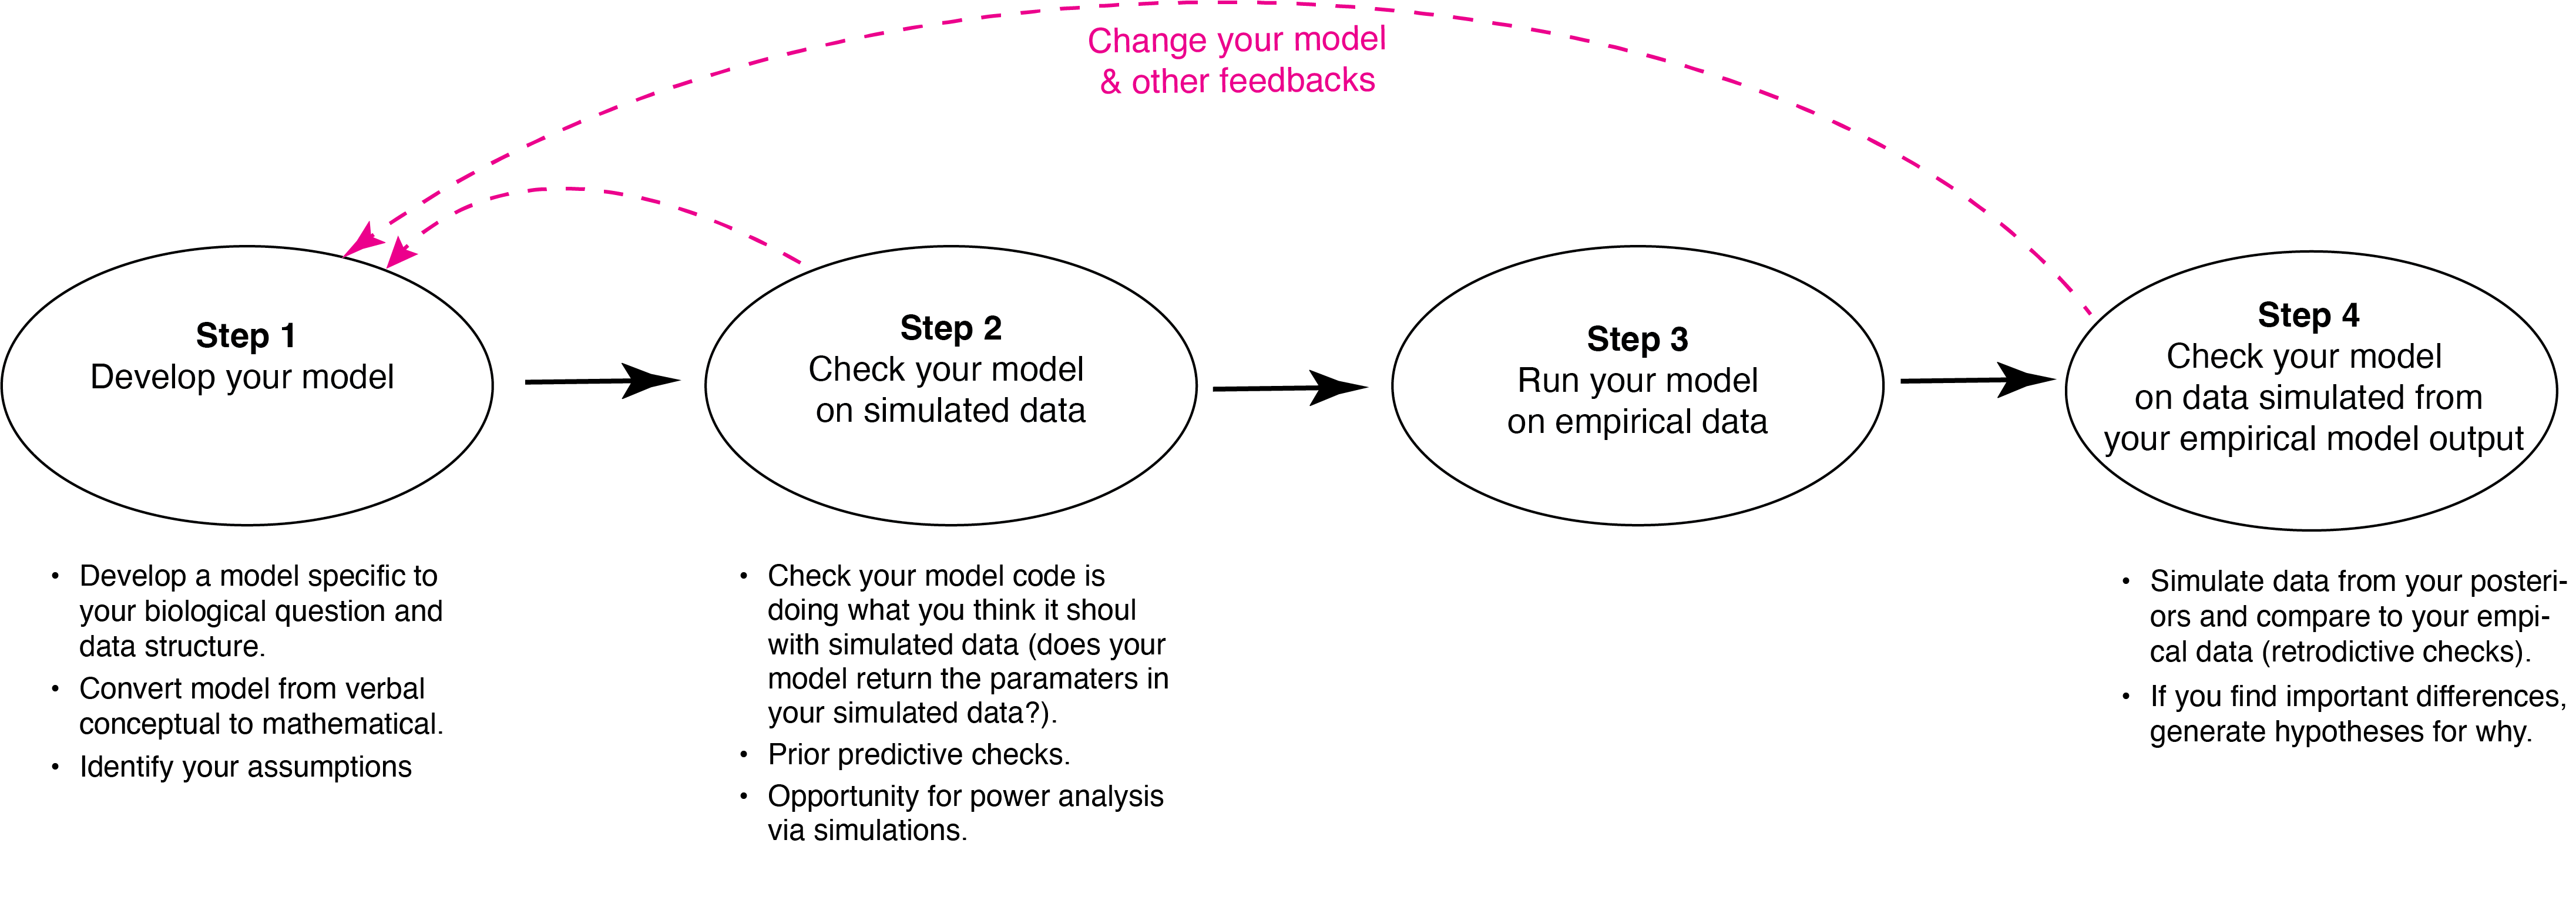
\includegraphics[width=0.7\textwidth]{figures/workflow.png}
\caption{A very basic workflow for Bayesian model fitting include four major steps with potential feedbacks (pink dashed arrows) and begins with testing your model through simulated (test) data.}
\label{fig:workflow}
\end{figure}

\begin{figure}[ht]
\centering
\noindent 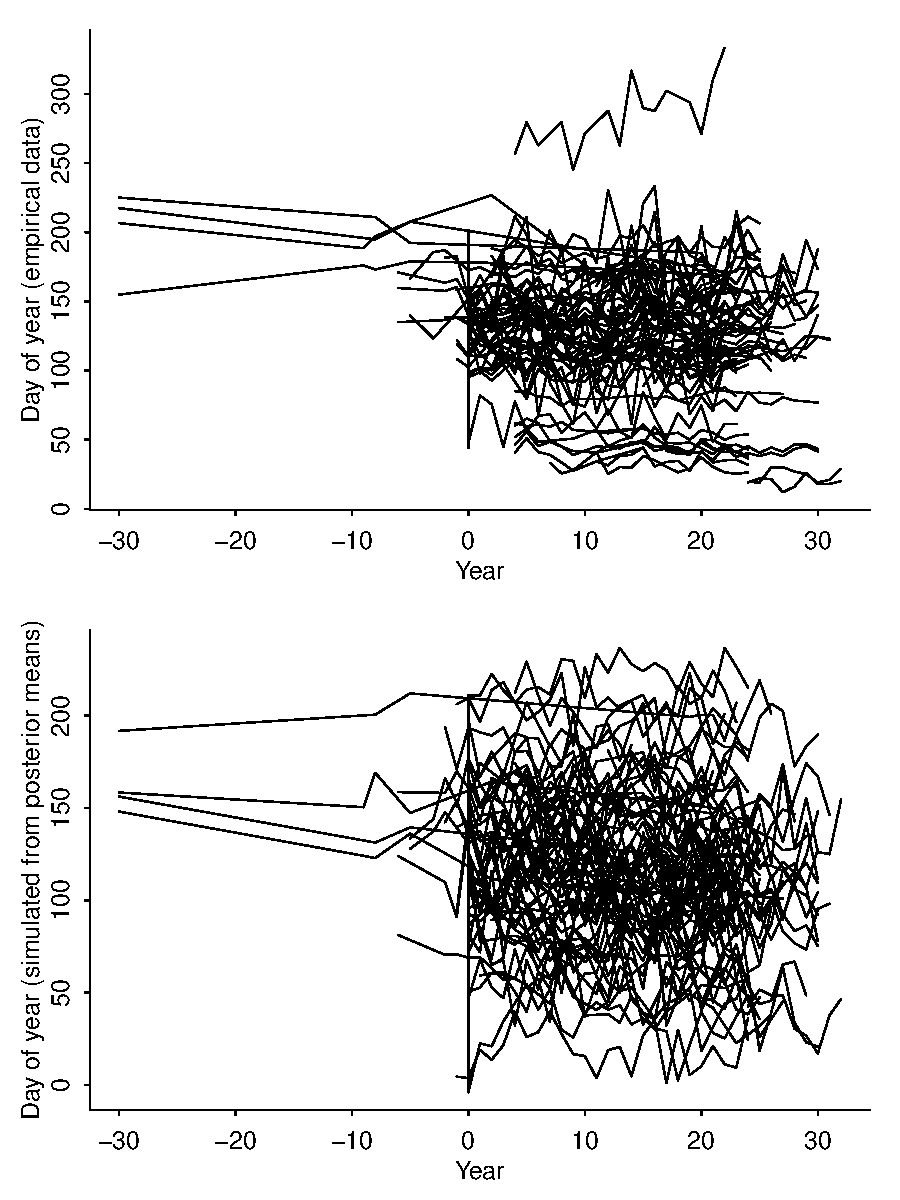
\includegraphics[width=0.8\textwidth]{examples/synchrony/graphs/rawvsonepredictivecheck.pdf}
\caption{Example of a retrodictive check from time-series data of phenological events over time (raw data on top; one simulated dataset on the bottom, based on existing species number and their respective $x$ data).}
\label{fig:retrodictivecheck}
\end{figure}

\begin{figure}[ht]
\centering
\noindent 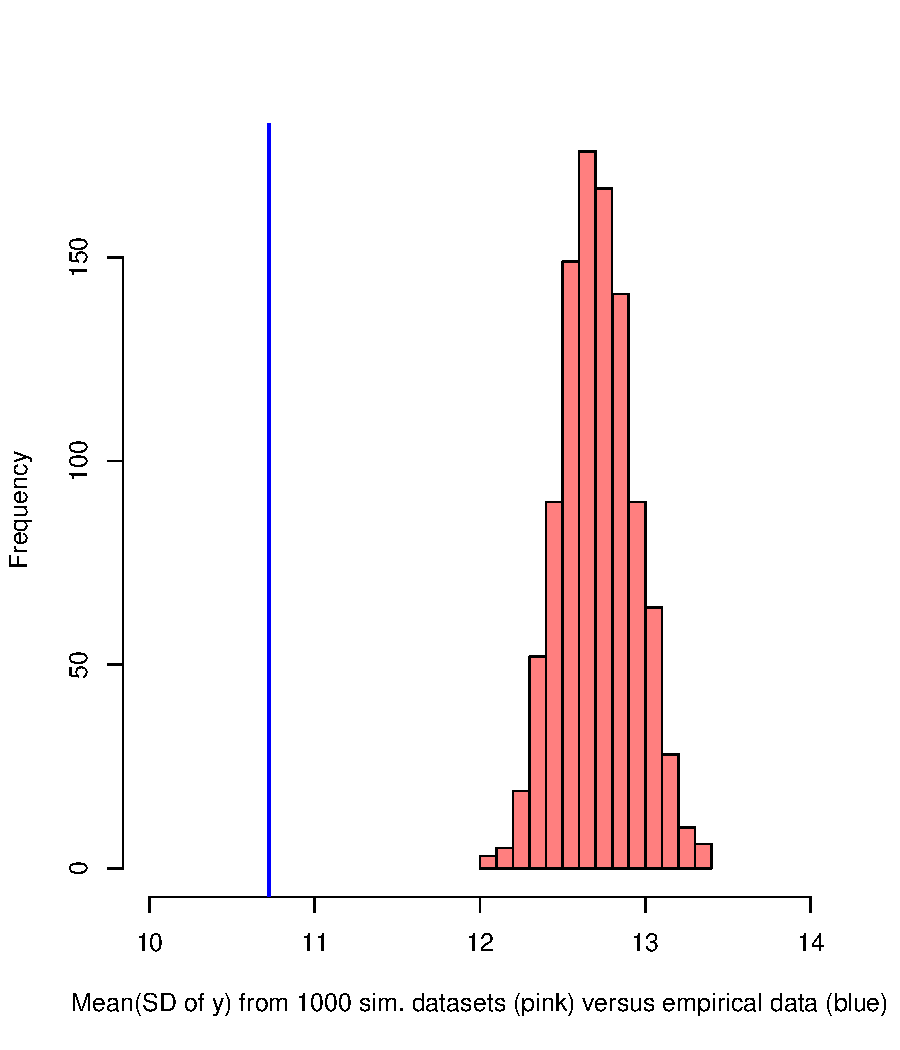
\includegraphics[width=0.5\textwidth]{examples/synchrony/graphs/retroSDsync.pdf}
\caption{Example of a retrodictive check from time-series data of phenological events over time, averaging across 1000 simulations.}
\label{fig:retrodictivecheckSD}
\end{figure}

\end{document}